\section{Problem Formulation}
\paragraph{Standard Inference} Denote the input prompt to the LLM as $\bm{x}=(x_1,x_2,...,x_{T})$, the standard generative inference process consists of two consecutive stages: prefilling and auto-regressive decoding. The prefilling stage encodes the input prompt $\bm{x}$ and produces the corresponding attention key matrix $\bm{K}_T\in \mathbb{R}^{L\times H\times T\times d^\prime}$ and value matrix $\bm{V}_T\in \mathbb{R}^{L\times H\times T\times d^\prime}$, 
where $L$, $H$, $d^\prime$ represent the number of model layers, number of attention heads, and per-head dimension, respectively. 
Afterward, the LLM samples one token from its output distribution at each step conditioned on all key-value states computed so far. The key-value matrices are updated by appending the key-value vectors of this new token:
\begin{align}
    x_{T+1}&\sim \text{LLM}(\cdot | x_{<=T}) \\
    \bm{K}_{T+1}&=\text{Concat}(\bm{K}_T, K_{T+1}) \\ 
    \bm{V}_{T+1}&=\text{Concat}(\bm{V}_T, V_{T+1})
\end{align}
where $K_{T+1}\in \mathbb{R}^{L\times H\times 1\times d^\prime}$, $V_{T+1}\in \mathbb{R}^{L\times H\times 1\times d^\prime}$ are the key and value vectors of $x_{T+1}$. 
The above process is repeated until the end of sequence token is generated. Let $\tilde{\bm{x}}=(\bm{x}, \bm{x}_o)$ denote the complete token sequence composed of input prompt $\bm{x}$ and output $\bm{x}_o$, where the output sequence contains $N$ tokens. 
The peak cache size during standard inference is therefore determined by the key-value matrix $\{\bm{K}_{T+N},\bm{V}_{T+N}\}\in \mathbb{R}^{L\times H\times (T+N)\times d^\prime}$.

\paragraph{Key-Value Constrained Inference}
LLMs are typically deployed on hardware with constrained memory resources. However, during standard generative inference, the size of the key-value cache increases linearly with the total length of the sequence, potentially leading to out-of-memory issues and the associated latency incurred by reading and writing between High Bandwidth Memory (HBM) and Static Random Access Memory (SRAM)~\cite{dao2022flashattention}.

To this end, recent studies have shifted toward key-value-constrained inference as a more controllable inference scheme. Denoting the fixed budget for each attention head as $B$ tokens, key-value constrained inference is to maintain the key-value matrices $\bm{K}_t$ and $\bm{V}_t$ such that 
$\bm{K}_t$, $\bm{V}_t\in \mathbb{R}^{L\times H\times n\times d^\prime}$ and $n\leq B$ for any $t\in\{1,...,T+N\}$. 

\section{Eviction Policy for Key-Value Constrained Inference}
In practice, $\bm{K}_t$ and $\bm{V}_t$ are stored in a fixed memory buffer with a maximum token budget $B$. When the buffer is full, an eviction policy is executed to remove stored but non-influential tokens from the cache. Although various eviction policies have been proposed, there still lacks a systematic comparison of their working mechanisms, design choices, and downstream performance. 

To fill this gap, we embark on the efficacy of existing eviction policies from a unified 
framework. Concretely, we represent an eviction policy as the composition of two components: 
importance score calculation and eviction scope construction, which we elaborate 
on in the following sections. 
\subsection{Importance Score Calculation}
\label{sec:isc}
Importance score calculation plays a vital role in eviction policy. It determines the relative order by which tokens are evicted. We summarize existing importance score calculation methods as follows: \\
\textbf{Random Deletion}~~As a naive baseline, one can randomly choose the key-value vectors to evict. We incorporate this method into comparison and let it serve as the lower bound. \\
\textbf{Recency}~~This method deems the farthest token as least important and evicts it when the buffer is full. It is also referred to as window attention in prior studies~\cite{etc,longformer,xiao2023efficient}. \\
\textbf{Accumlative Attention Score~(AAS)}~~$\text{H}_{\text{2}}$O~\cite{h2o} maintains a $B$-sized record array that stores the accumulative attention score each in-cache token received from subsequent tokens. \\
\textbf{Accumlative Quantized Attention Score~(AQAS)}~~ScissorHands~\cite{liu2023scissorhands} adopts an apporach similar to $\text{H}_{\text{2}}$O. The exception is that the attention score is quantized into a binary value, with 1 indicating above average and 0 indicating below average. \\
\textbf{Last Token Attention Score~(LTAS)}~~TOVA~\cite{tova} uses last token's attention score as importance indicator.

\subsection{Eviction Scope Construction}
\label{sec:esc}
Due to the auto-regressive nature of LLMs, recent tokens in the cache participate in less attention computation than earlier tokens. Therefore, their recorded importance scores for some attention-based methods can be underestimated and thus get wrongly evicted. To this end, an eviction scope should be constructed to carefully select tokens allowed to be evicted.

The dominant mean of constructing eviction scope is 
 \textit{\textbf{local window}}, which assumes that tokens outside of a 
local window of size $r$ have accumulated sufficient information on their importance.

\subsection{Preliminary Experiments}
\label{sec:preliminary}
In our controlled preliminary experiments, we are interested in how different importance 
score calculation methods behave in terms of consistency with respect to 
their full KV cache version. After that, we also explore another way of constructing 
eviction scope in addition to local window.

\begin{figure}[t]
	\centering
	\scalebox{0.415}{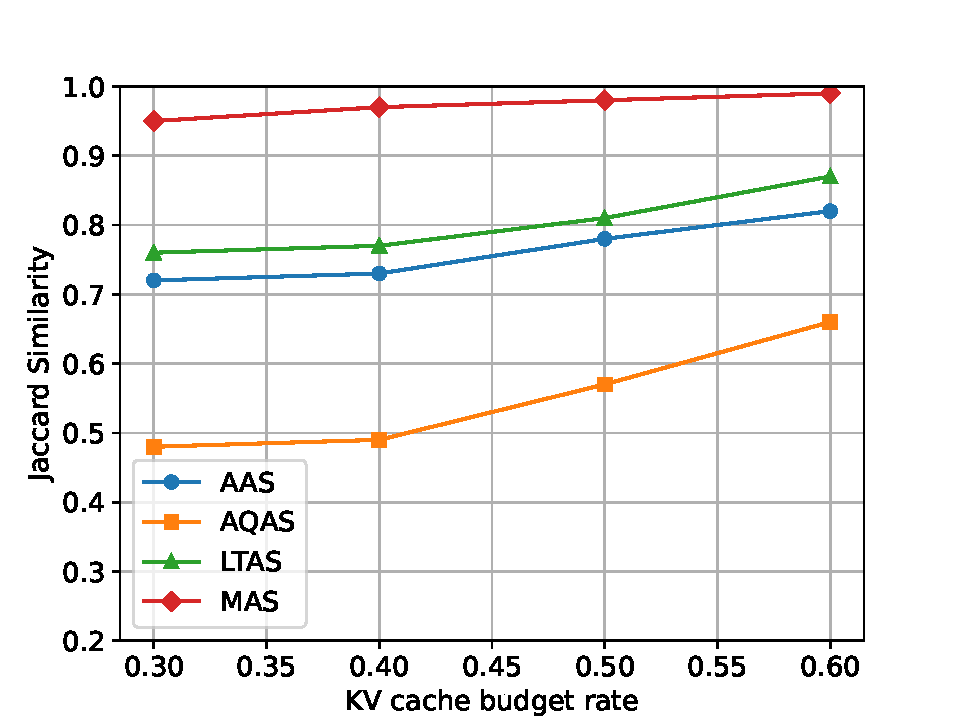
\includegraphics{./figures/consistency.pdf}}
	\caption{Consistency of different importance calculation methods w.r.t their full KV cache variant.}
	\label{fig:consistency}
\end{figure}

\paragraph{Setup} We examine the Jaccard similarity between the top-$B$ important tokens 
derived by various importance score calculation methods and those derived when a full 
KV cache is available. The higher the similarity, the more effectively the importance 
calculation method harnesses local information to approximate the global one. We evaluate all 
attention-based methods~(i.e., AAS, AQAS, and LTAS) listed in \secref{sec:isc} and set 
the local window size $r$ to 0. More specifically, we use LLaMa2-7B-Chat\footnote{We also 
conduct experiments upon other LLMs like WizardLM-7B, and similar results are observed.} as the LLM and take the 805 instructions from AlpacaEval~\cite{alpaca_eval} as prompt, generating a response for each instruction via greedy decoding. For KV cache budget from $\{0.3,0.4,0.5,0.6\}$, we compute the Jaccard similarity at each token position, averaged over sequence length, attention heads, and layers. 

\paragraph{Results} The results are shown in \figref{fig:consistency}. AAS shows a clear advantage over AQAS across all budget rates, indicating the importance of a full-precision attention score when the relative importance of tokens cannot be distinguished via binary value. LTAS has higher consistency than AAS, which we attribute to the fact that 
LTAS does not suffer from the recency bias that AAS and AQAS exhibit due to the accumulation operation. However, LTAS computes importance score based on a single token, which might bear high variability. Based on the above results, we advocate the use of \textit{Mean Attention Score~(MAS) to gauge the importance of each token}. MAS divides each token's accumulative attention score by how many times that token is attended by future tokens. As shown in \figref{fig:consistency}, MAS has remarkably higher consistency among all methods, achieving over 0.9 Jaccard similarity even at 0.3 cache budget rate. This verifies that MAS effectively alleviates recency bias and can better retain high-influential tokens.
\begin{figure}[t]
	\centering
	\scalebox{0.48}{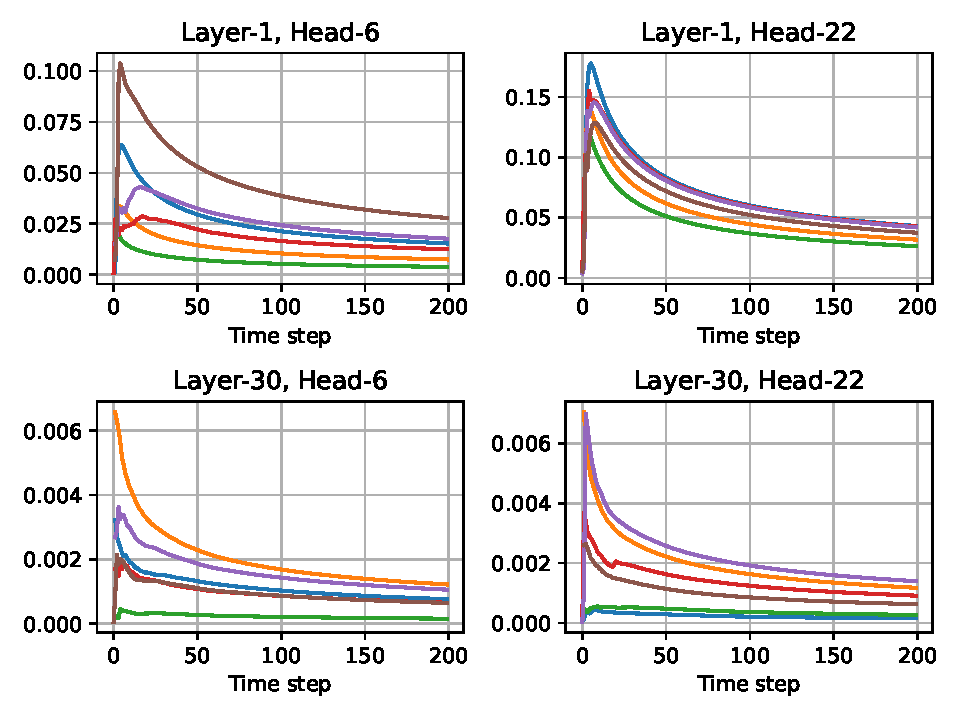
\includegraphics{./figures/std.pdf}}
    \caption{Illustration of persistence of attention robustness. We extract attention scores and compute the standard deviation from LLaMa2-7B-Chat.}
	\label{fig:std}
\end{figure}

\paragraph{Is Local Window the Optimal Way to Construct Eviction Scope?} 
The local window approach has been widely used in conjunction with attention-based importance calculation methods to prevent recent tokens from being evicted. The underlying rationale is that the accumulated attention score is not sufficiently indicative until a specified threshold, i.e., the window size $r$ is reached. 

Based on the commendable consistency of MAS discussed in the previous paragraph, here we propose another way to construct the eviction scope which exploits a phenomenon termed \textit{persistence of attention robustness} that we find ubiquitously exists in large language models.  
It states that the standard deviation of the attention probabilities a token receives 
from future tokens typically undergoes a brief ascending phase before settling into a stable 
decline, regardless of the model layer and attention head. \figref{fig:std} clearly illustrates the phenomenon. We also observe that the ascending phase of a non-trivial portion of tokens only takes a relatively small number of steps, i.e., $\leq 50$, suggesting it might be sub-optimal to only consider tokens at least $r$ steps away for eviction scope construction. 

To this end, we propose a new way to construct the eviction scope utilizing the \textit{standard deviation} of attention scores. Concretely, we maintain another $B$-sized array for each attention head, keep track of the accumulative squared attention score, and compute the standard deviation of each in-cache token $x$ using $\text{Std}(x)=\sqrt{\frac{\text{Acc}^{\text{square}}(x)}{\text{Count}(x)}-(\frac{\text{Acc}(x)}{\text{Count}(x)})^2}$. In practice, Acc, Acc$^{\text{sqaure}}$, and Count are all $B$-sized tensor and the standard deviation of all in-cache tokens are computed in parallel. Then, instead of the most recent $r$ tokens, we exclude tokens having top-$r$ standard deviation from eviction scope and remove the key-value vectors corresponding to the token with the lowest mean attention score. 

\begin{figure}[t]
	\centering
	\scalebox{0.385}{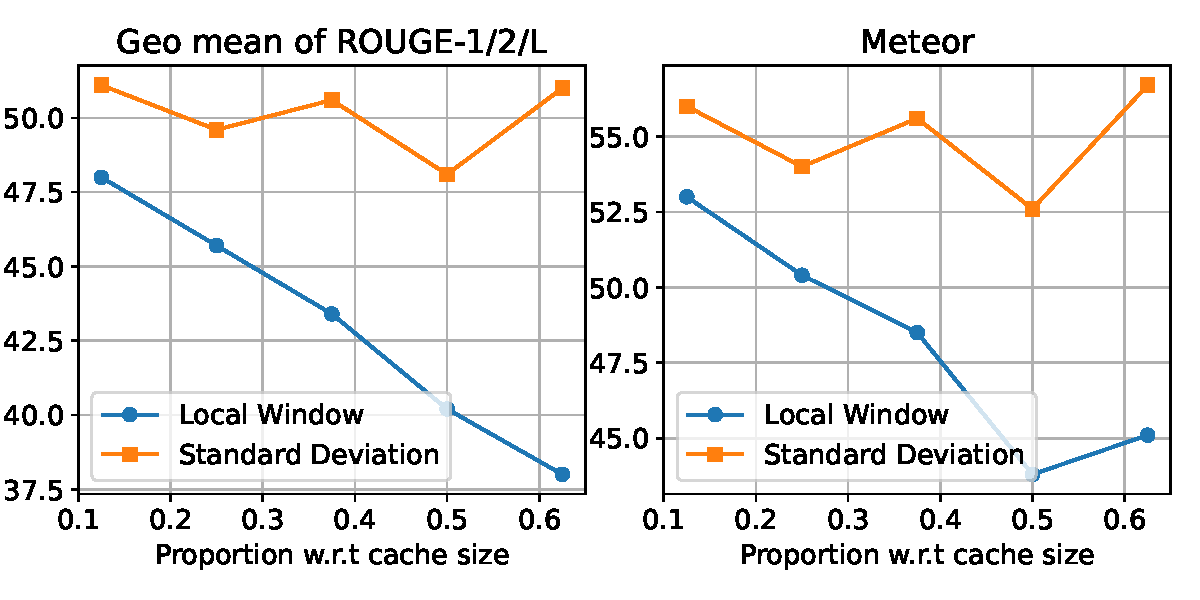
\includegraphics{./figures/scope.pdf}}
    \caption{Results of MAS paired with local window and standard deviation on text summarization.}
	\label{fig:scope}
\end{figure}
We validate the effectiveness of both eviction scopes on a news summarization task with LLaMa2-7B-Chat and CNN/Daily Mail~\cite{cnndm} dataset. Since summarization is a typical long-input-short-output task, we only perform KV eviction at the prefilling stage with a 0.5 compression rate and compare the output against the full KV cache version. \figref{fig:scope} shows the geometric mean of ROUGE-1/2/L~\cite{rouge} and METEOR~\cite{meteor} for eviction scopes of different sizes. Standard deviation yields outputs with considerably higher quality while being less sensitive to the size of the eviction scope.

\paragraph{RoCo} Combining mean attention score for importance score calculation and standard deviation for eviction scope construction, we introduce RoCo as a \underline{R}\underline{o}bust \underline{C}ache \underline{o}mission policy for key-value constrained generative LLM inference.
